%%% Thesis Introduction --------------------------------------------------
\chapter{Introduction}

\graphicspath{ {Introduction/IntroductionFigs/PNG/}
  {Introduction/IntroductionFigs/PDF/}
  {Introduction/IntroductionFigs/} }

La modélisation géométrique a permis, dans un premier temps, de
représenter des modèles virtuels. De ce fait, des outils permettant la
modification de ces modèles se sont directement mis en place, au
travers du déplacement des différents sommets des modèles. Mais
d'autres types de déformation se sont instaurées par la suite, comme
la déformation \textit{spatiale}.
\\

La déformation spatiale consiste à déformer un objet en modifiant son
espace ambiant.  On notera \cite{Bar84} et \cite{SP86} comme étant les
premiers à avoir introduit ce type de déformation. Ce procédé a un
avantage considérable, la modification de l'espace. En effet comme la
déformation est réalisée sur chaque point de l'espace de façon
indépendante, elle n'est pas liée à la représentation interne de
l'objet. Cette propriété est essentielle, car elle permet d'assurer
que, peu importe la topologie existante entre les points de l'espace à
déformer, une même déformation de l'outil déformera l'espace de la
même manière.
\\

La première partie de ce travail consiste en la réalisation d'un
mélange de multiples outils de déformation. En parallèle, une étude
est faite sur les outils de déformation de différentes dimensions,
pour déterminer le meilleur outil associé à chaque dimension (point,
courbe, surface, volume). Au final il s'agira de pouvoir obtenir une
génération automatique d'un outil multidimensionnel de déformation
associé à un modèle, en segmentant ce dernier et en associant à
chacune de ses segmentations l'outil de déformation le plus adapté à
sa forme.
\\

On voudrait, pour un même modèle, associer des outils bien précis à
certaines parties de ce modèle. Prenons le modèle de l'alligator
(Figure \ref{INTall}), on souhaiterait ouvrir la bouche de
l'alligator, élargir son ventre et bouger sa queue, mais ce n'est pas
possible avec un seul outil. L'idée serait alors d'appliquer des
outils différents sur plusieurs zones d'un objet, ou différents outils
sur une même zone. En reprenant l'exemple de l'alligator, il faudrait,
pour avoir le comportement décrit plus-haut, associer des points pour
la queue, des axes pour la bouche et une cage pour le ventre. On se
demande alors comment mélanger ces outils de façon à ce que les
déformations se fassent de manière continue (à interpréter tout au
long du travail par une continuité $C^1$ au moins), et de quelle
manière délimiter la zone d'influence de chaque outil, afin que la
déformation appliquée par un outil se fasse dans une zone limitée. De
plus, il faut s'assurer que tous les outils peuvent définir des
coordonnées de façon continue dans ces "zones d'influence". En effet,
car si les outils de déformation de dimension topologique 0 et 1
(c'est-à-dire points et courbes respectivement) appliquent une
déformation dans une zone autour d'eux, les outils de dimension 2 et 3
(surfaces et volumes) ne déforment que la zone de l'espace contenue en
leur intérieur (ou en leur extérieur) de façon continue, mais le
passage de l'extérieur à l'intérieur n'est pas continu autour des
sommets (uniquement $C^0$).
\\


\begin{figure}[h]
  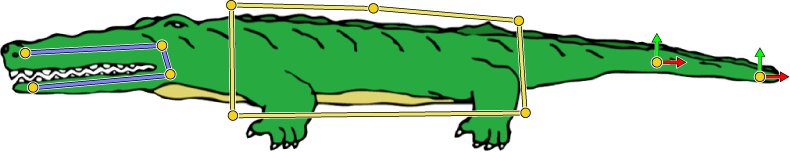
\includegraphics[scale=0.25]{alligator-avant}
  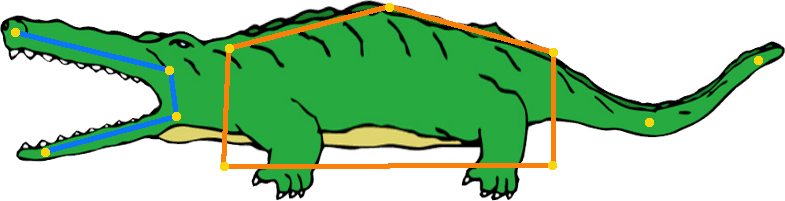
\includegraphics[scale=0.25]{alligator-apres}
  \caption{A gauche le modèle d'origine et à droite le modèle après
    déplacement de certains points de contrôle}
  \label{INTall}
\end{figure}

De plus, en fonction de la précision de la déformation à appliquer, il
serait intéressant de pouvoir disposer de plusieurs niveaux de
résolution pour les différents outils utilisés, afin de pouvoir avoir
un plus grand nombre de degrés de liberté lors d'une déformation
précise, et un plus faible lors d'une déformation plus globale. Mais
de ce fait, il faut mettre en place un moyen de faire communiquer les
différents niveaux de résolution entre eux, comme le modèle proposé
par \cite{Hur12} concernant les déformation à base de cages.
\\

Tout au long de ce travail, nos choix ont été motivés par la volonté
de fournir un outil permettant de déformer des points de l'espace de
manière interactive et fluide, et d'obtenir des formulations
mathématiques simples et claires. Le but de ce travail est de
permettre à un utilisateur d'obtenir un outil de déformation
s'adaptant à ses besoins, en générant de façon automatique un outil
multidimensionnel de déformation, tout en lui laissant la possibilité
de paramétrer le comportement des différents outils utilisés.
%%% ----------------------------------------------------------------------


%%% Local Variables: 
%%% mode: latex
%%% LaTeX-command: "latex -shell-escape"
%%% TeX-master: "../thesis"
%%% End: 
